%%%%%%%%%%%%%%%%%%%%%%%%%%%%%%%%%%%%%%%%%
% Jacobs Portrait Poster
% LaTeX Template
% Version 1.0 (31/08/2015)
% (Based on Version 1.0 (29/03/13) of the landscape template
%
% Created by:
% Computational Physics and Biophysics Group, Jacobs University
% https://teamwork.jacobs-university.de:8443/confluence/display/CoPandBiG/LaTeX+Poster
% 
% Further modified by:
% Nathaniel Johnston (nathaniel@njohnston.ca)
%
% Portrait version by:
% John Hammersley
%
% The landscape version of this template was downloaded from:
% http://www.LaTeXTemplates.com
%
% License:
% CC BY-NC-SA 3.0 (http://creativecommons.org/licenses/by-nc-sa/3.0/)
%
%%%%%%%%%%%%%%%%%%%%%%%%%%%%%%%%%%%%%%%%%

%----------------------------------------------------------------------------------------
%	PACKAGES AND OTHER DOCUMENT CONFIGURATIONS
%----------------------------------------------------------------------------------------

\documentclass[final]{beamer}
\usepackage[explicit]{titlesec}
\usepackage{ulem}
\usepackage[scale=1.24]{beamerposter} % Use the beamerposter package for laying out the poster

\usetheme{confposter} % Use the confposter theme supplied with this template

\setbeamercolor{block title}{fg=ngreen,bg=white} % Colors of the block titles
\setbeamercolor{block body}{fg=black,bg=white} % Colors of the body of blocks
\setbeamercolor{block alerted title}{fg=white,bg=dblue!70} % Colors of the highlighted block titles
\setbeamercolor{block alerted body}{fg=black,bg=dblue!10} % Colors of the body of highlighted blocks
% Many more colors are available for use in beamerthemeconfposter.sty

%-----------------------------------------------------------
% Define the column widths and overall poster size
% To set effective sepwid, onecolwid and twocolwid values, first choose how many columns you want and how much separation you want between columns
% In this template, the separation width chosen is 0.024 of the paper width and a 4-column layout
% onecolwid should therefore be (1-(# of columns+1)*sepwid)/# of columns e.g. (1-(4+1)*0.024)/4 = 0.22
% Set twocolwid to be (2*onecolwid)+sepwid = 0.464
% Set threecolwid to be (3*onecolwid)+2*sepwid = 0.708

\newlength{\sepwid}
\newlength{\onecolwid}
\newlength{\twocolwid}
\newlength{\threecolwid}
\setlength{\paperwidth}{36in} % A0 width: 46.8inProve that any direct quantum link in protocols can be replaced by its teleportation implementation without re-proving security 

\setlength{\paperheight}{48in} % A0 height: 33.1in
\setlength{\sepwid}{0.024\paperwidth} % Separation width (white space) between columns
\setlength{\onecolwid}{0.20\paperwidth} % Width of one column
\setlength{\twocolwid}{0.352\paperwidth} % Width of two columns
\setlength{\threecolwid}{0.598\paperwidth} % Width of three columns
\setlength{\topmargin}{-1.7in} % Reduce the top margin size
%-----------------------------------------------------------

\usepackage{graphicx}  % Required for including images

\usepackage{booktabs} % Top and bottom rules for tables

%----------------------------------------------------------------------------------------
%	TITLE SECTION 
%----------------------------------------------------------------------------------------

\title{Composing entanglement distillation and teleportation for cryptographic applications
} % Poster title


\author{Harold Ollivier$^{1}$, Rhea Parekh$^{1, 2}$} % Author(s)


\institute{$^{1}$ LIP6, CNRS, Sorbonne Universit\'e, France, $^{2}$ Department of Physics, Indian Institute of Technology, Roorkee, India} % Institution(s)

%----------------------------------------------------------------------------------------

\begin{document}

\addtobeamertemplate{block end}{}{\vspace*{2ex}} % White space under blocks
\addtobeamertemplate{block alerted end}{}{\vspace*{2ex}} % White space under highlighted (alert) blocks

\setlength{\belowcaptionskip}{2ex} % White space under figures
\setlength\belowdisplayshortskip{2ex} % White space under equations

\begin{frame}[t] % The whole poster is enclosed in one beamer frame

\begin{columns}[t] % The whole poster consists of three major columns, the second of which is split into two columns twice - the [t] option aligns each column's content to the top

\begin{column}{\sepwid}\end{column} % Empty spacer column

\begin{column}{\onecolwid} % The first column

%----------------------------------------------------------------------------------------
%	OBJECTIVES
%----------------------------------------------------------------------------------------

\begin{alertblock}{Context}

\begin{itemize}
\item Quantum internet prototypes are being defined and tested, Their goal is to demonstrate a decisive advantage of classical networks.
\item Network layer models \cite{Wehnereaam9288} are proposed to define elementary functionalities for extending networks piece-wise and to describe protocols using higher-level abstractions.
\item Most works take bottom-up approaches where layers are defined starting from physical constraints.
\end{itemize}
In this work, we advocate for a top-down approach to network layer model definition as a way to achieve security by design and demonstrate how quantum-links can be securely defined and analyzed.
\end{alertblock}

%----------------------------------------------------------------------------------------
%	INTRODUCTION
%----------------------------------------------------------------------------------------

\begin{block}{What’s at stake}

\begin{itemize}
\item We are at a decisive moment: Networks are being prototyped, it is a unique opportunity to adjust our models before it becomes too costly.
\item We build over the shortcomings of classical networks: Security shall be a concern at all stages of network design, and not only at the application layer.
\item A secure network layers model needs to be worked out.
\end{itemize}

\end{block}

\begin{block}{Proposal}

\begin{itemize}
\item Extract reusable functions from protocols that can be plugged into advanced functionalities.
\item Use abstract cryptography \cite{Maurer11abstractcryptography} and universal composability as frameworks to combine reusable functions (resources) to achieve other secure, higher-order, functionalities.
\item Define a network layer model consistent with this approach.

\end{itemize}
\end{block}
%-----------------------------------------------
%----------------------------------------------------------------------------------------

\end{column} % End of the first column

\begin{column}{\sepwid}\end{column} % Empty spacer column

\begin{column}{\twocolwid} % Begin a column which is two columns wide (column 2)

\begin{columns}[t,totalwidth=\twocolwid] % Split up the two columns wide column

\begin{column}{\twocolwid}\vspace{-.6in} % The first column within column 2 (column 2.1)

%----------------------------------------------------------------------------------------
%	MATERIALS
%----------------------------------------------------------------------------------------
\begin{block}{Elementary functions: using Quantum Protocol Zoo}

\begin{figure}
   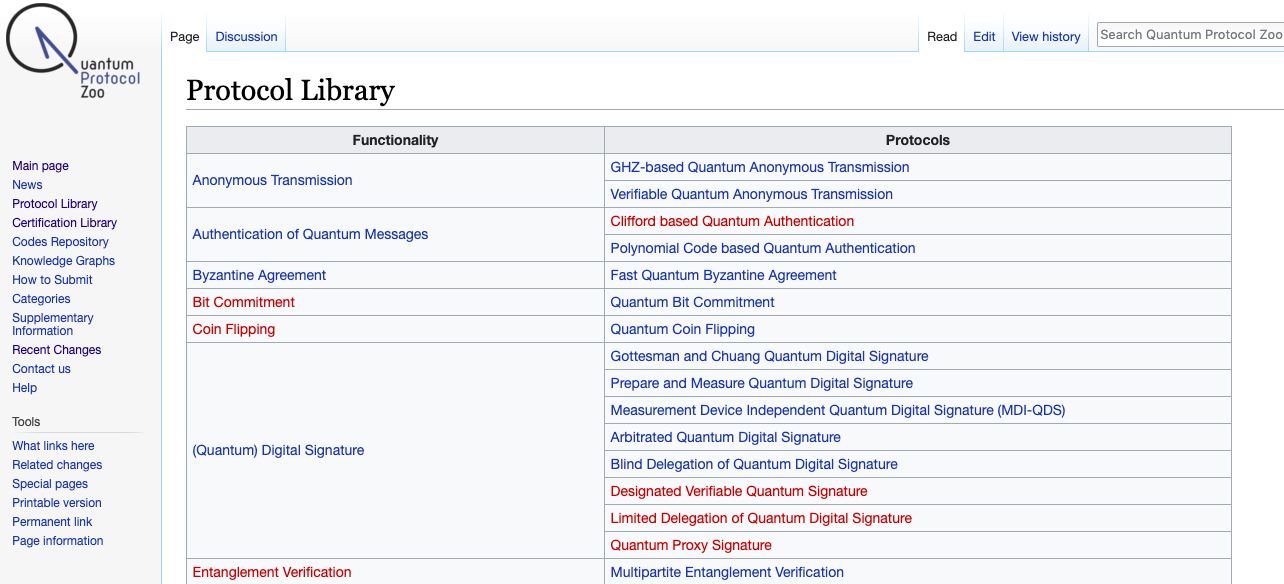
\includegraphics[width=0.90\linewidth]{Protocol_Zoo.png}
\end{figure}

\begin{itemize}
\item Using wiki.veriqloud.fr repository, it is possible to identify elementary resources that are used across many protocols.
\item Elementary functions need to be proven composable (i.e it is legitimate to use them as a “block” without reproving the security of the whole protocol using them)


\end{itemize}
\end{block}


\begin{block}{Direct quantum link through teleportation}
   \begin{itemize}
       \item A direct quantum link is a resource which connects two end points and allows to send a qubit from one to the other.
       \item Current technology is limiting our ability to transmit quantum information (probabilistic emission events and high losses).
      \item Our goal is to: Construct this resource by using quantum teleportation as it is more reliable and prove that any direct quantum link in protocols can be replaced by its teleportation implementation without re-proving security.

   \end{itemize}
 
 
   \begin{columns}
     \begin{column}{.60\textwidth}
        \begin{itemize}
       \item The ideal functionality allows E to temper with quantum messages  
       \item The teleportation implementation uses a perfect EPR pair that E can substitute
   \end{itemize}
     \end{column}%
    \hfill%
    
     \begin{column}{.40\textwidth}
        \begin{figure}
         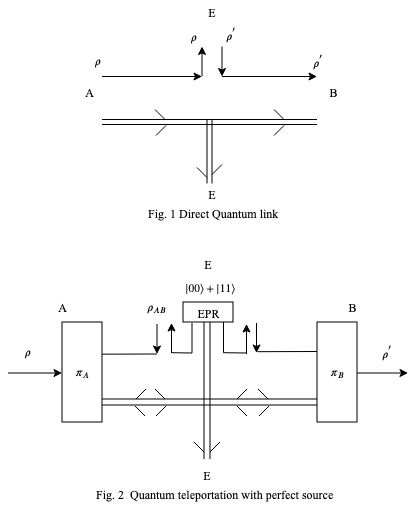
\includegraphics[width=0.95\linewidth]{direct_quantum_link.jpg}
       \end{figure}
     \end{column}%
   \end{columns}
  \vskip 1cm  
 
  \begin{columns}
   
    \begin{column}{.40 \textwidth} % Right column and width
        \centering
       \begin{figure}
         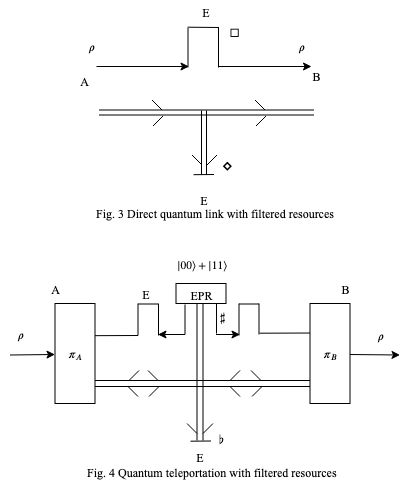
\includegraphics[width=0.95\linewidth]{direct_quantum_link_filtered.jpg}
       \end{figure}
    \end{column}
    \hfill%
     \begin{column}{.60\textwidth} % Left column and width
       \centering
       \textbf{Correctness}\\[.2cm]
       
       \begin{itemize}
           \item Correctness is equivalent to showing that teleportation allows to send 1 qubit in absence of malicious behavior in E.
       \end{itemize}
    \end{column}%
  \end{columns}
  
  \vskip 2cm
  \begin{columns}
  
    \begin{column}{.60 \textwidth} % Right column and width
        \centering
       \textbf{Security}\\[.2cm]
       \begin{itemize}
           \item We define a simulator that will “fake” teleportation and use an ideal direct quantum link instead
          \item Both settings (teleportation based and ideal + simulator) are indistinguishable thus proving the security
       \end{itemize}
    \end{column} 
    \hfill%
    \begin{column}{.40\textwidth} % Left column and width
       \centering
       \begin{figure}
         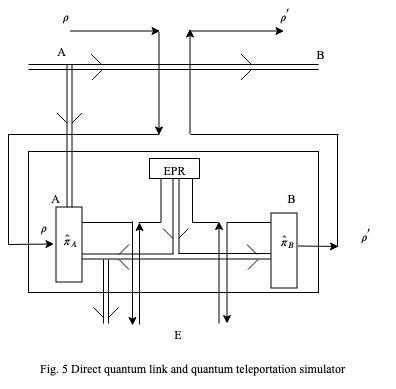
\includegraphics[width=0.95\linewidth]{direct_quantum_link_simulator.jpg}
       \end{figure}
    \end{column}%
  \end{columns}

\end{block}

%----------------------------------------------------------------------------------------

\end{column} % End of column 2.1

\begin{column}{\onecolwid}\vspace{-.6in} % The second column within column 2 (column 2.2)

%----------------------------------------------------------------------------------------
%	METHODS
%----------------------------------------------------------------------------------------



%----------------------------------------------------------------------------------------

\end{column} % End of column 2.2

\end{columns} % End of the split of column 2 - any content after this will now take up 2 columns width

%----------------------------------------------------------------------------------------
%	IMPORTANT RESULT
%----------------------------------------------------------------------------------------
%----------------------------------------------------------------------------------------


\end{column} % End of the second column

\begin{column}{\sepwid}\end{column} % Empty spacer column

\begin{column}{\twocolwid} % The third column

%----------------------------------------------------------------------------------------
%	CONCLUSION
%----------------------------------------------------------------------------------------

\begin{block}{EPR source through entanglement distillation}

\begin{itemize}
    \item Perfect heralded EPR sources do not exist
    \item Entanglement distillation is taking imperfect pairs and turning them into better ones
\end{itemize}

\begin{columns}
    \begin{column}{.60\textwidth}
       \begin{itemize}
          \item A and B run 3 stage protocols designed to allow correct and secure distillation \cite{Pirker_2017}
          \item Stage 1: Twirl + Symmetrization
          \item Stage 2: Fidelity verification
          \item Stage 3: Entanglement distillation 
        \end{itemize}
    \end{column}%
    \hfill%
    
    \begin{column}{.40\textwidth}
        \begin{figure}
         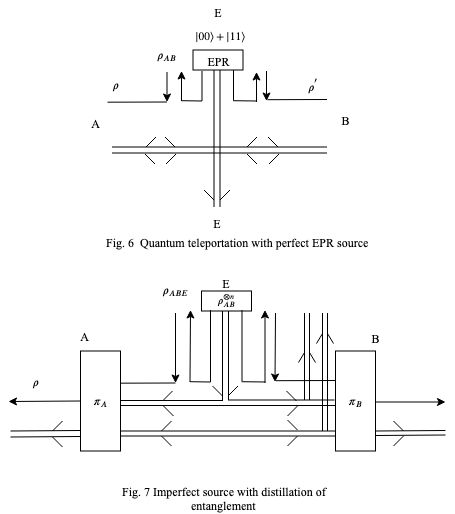
\includegraphics[width=0.95\linewidth]{direct_quantum_link_imperfect.jpg}
       \end{figure}
    \end{column}%
\end{columns}

\vskip 2cm 

\begin{columns}
    \begin{column}{.40\textwidth}
       \begin{figure}
         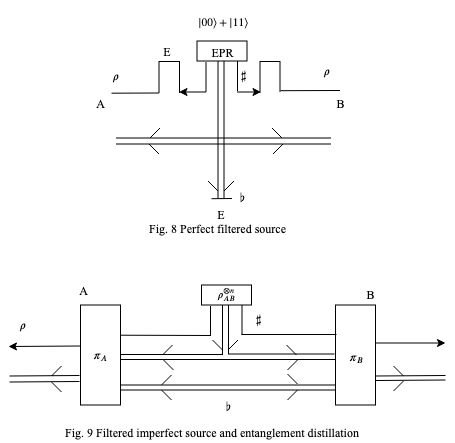
\includegraphics[width=0.95\linewidth]{direct_quantum_link_imperfect_filtered.jpg}
       \end{figure}
    \end{column}%
    
    \hfill%
    
    \begin{column}{.60\textwidth}
       \centering
       \textbf{Correctness}\\[.2cm]
       $\epsilon$-correctness follows from:
       \begin{itemize}
           \item Twirl + Symmetrization providing i.i.d. pairs
           \item Approximate fidelity verification for picking the right distillation algorithm with high probability
           \item Almost always succeeding distillation 
       \end{itemize}
    \end{column}%
\end{columns}

\vskip 2cm 

\begin{columns}
    \begin{column}{.60\textwidth}
        \centering
       \textbf{Security}\\[.2cm]
       $\epsilon$-security relies on:
       \begin{itemize}
           \item Simulators that reliably detects states with low fidelity which would derail distillation
          \item Distillation protocols that produce high purity pairs such that any engineered correlation between sent pairs and the distinguisher would be washed away (monogamy of entanglement / gentle measurement theorem)
         \end{itemize} 
    \end{column}%
    
    \hfill%
    
    \begin{column}{.40\textwidth}
       \begin{figure}
         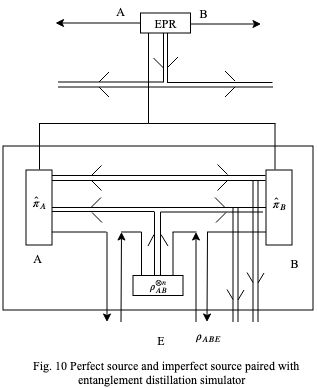
\includegraphics[\linewidth]{direct_quantum_link_imperfect_simulator.jpg}
       \end{figure}
    \end{column}%
\end{columns}
\end{block}




%----------------------------------------------------------------------------------------
%	REFERENCES
%----------------------------------------------------------------------------------------

\begin{block}{References}

\nocite{*} % Insert publications even if they are not cited in the poster
\small{\bibliographystyle{ieeetr}
\bibliography{sample}}

\end{block}

%----------------------------------------------------------------------------------------
%	ACKNOWLEDGEMENTS
%----------------------------------------------------------------------------------------

\setbeamercolor{block title}{fg=red,bg=white} % Change the block title color

\begin{block}{Acknowledgements}

\small{\rmfamily{The authors acknowledge financial support from the ANR International Project VanQute; the European Union’s Horizon 2020 Research and Innovation Programme under Grant Agreement  No. 820445 (QIA); The UK Engineering and Physical Sciences Research Council Grant No. EP/N003829/1 as well as technical supports from VeriQloud for hosting the Zoo.}} \\

\end{block}

%----------------------------------------------------------------------------------------
%	CONTACT INFORMATION
%----------------------------------------------------------------------------------------

\setbeamercolor{block alerted title}{fg=black,bg=norange} % Change the alert block title colors
\setbeamercolor{block alerted body}{fg=black,bg=white} % Change the alert block body colors

\begin{block}{Contact Information}

\begin{itemize}
\item Web: \href{https://wiki.veriqloud.fr/index.php}{https://wiki.veriqloud.fr}
\item Email: \href{mailto:harold.ollivier@linksights.io}{harold.ollivier@linksights.io}
\end{itemize}

\end{block}


%----------------------------------------------------------------------------------------

\end{column} % End of the third column

\end{columns} % End of all the columns in the poster

\end{frame} % End of the enclosing frame

\end{document}
